\documentclass{article}
\usepackage[utf8]{inputenc}

\usepackage{ifxetex}
\ifxetex
  \usepackage{fontspec}
\else
  \usepackage[T1]{fontenc}
  \usepackage[utf8]{inputenc}
  \usepackage{lmodern}
\fi

\title{Reporte de Actividad 4}
\author{Roberto Benard Orci}
\date{21/02/2018}

\begin{document}
\maketitle

\section{Introducción}
En esta actividad trabajamos con Bourne Again Shell ($\backslash$bin$\backslash$bash) para aprender a hacer programas (scripts) interpretes de comandos que recompilen, junten y clasifiquen informacion de manera automatizada.
 
Un Shell script es un programa que recibe lo que se escribe en la terminal y lo convierte en instrucciones para el sistema operativo. Se denomina shell porque es la capa más externa alrededor del núcleo del sistema operativo.

\section{Actividad}

Lo primero que hicimos fue descargar un script que entra a la página de U. de Wyoming para descargar los datos clima de una región en un año en 12 archivos, uno para cada mes. Después cambiamos el número de estación de manera que los datos que descargara el script fueran los datos de la misma región que escogimos la practica pasada. 

Finalmente probamos diferentes comandos que nos servirían para organizar, ver y filtrar archivos. Con la intención de usar estos comandos en un script que automatizara el proceso de organizar y filtrar los archivos.

\section*{Comandos utilizados}

A continuación, daré una breve descripción sobre los comandos usados en esta práctica, estos están organizados en 3 secciones, los comandos se encuentran en la sección que mejor los describe aunque varios de estos comandos podrían estar en varias secciones a la vez.

\subsubsection*{echo}
Este comando sirve para escribir algo desde la terminal a un archivo o viceversa.

\begin{center}
	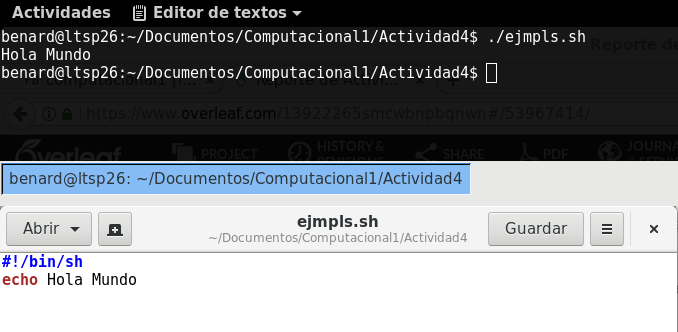
\includegraphics[width=12cm]{echo.png}
\end{center}
\vspace{0.3cm}

\subsection*{Obtención de datos}

\subsubsection*{grep}
Este comando tiene una gran cantidad de funciones, pero en esta práctica fue usado principalmente para descargar archivos en línea y para filtrar datos.

\subsection*{Organización de archivos}

\subsubsection*{pwd}
Sirve para obtener la ruta en donde se encuentra uno.

\subsection*{Herramientas para ver/filtrar contenido}

\subsubsection*{chmode}
Sirve para cambiar el acceso a un archivo para el usuario y demás usuarios, la "libertad" que tienen ver, leer y/o modificar el archivo.

\subsubsection*{ls -alg}
\textit{chmode} es el que cambia el acceso, \textit{ls - alg} es el que te muestra estas "libertades" de todos los archivos de una carpeta.

\begin{center}
	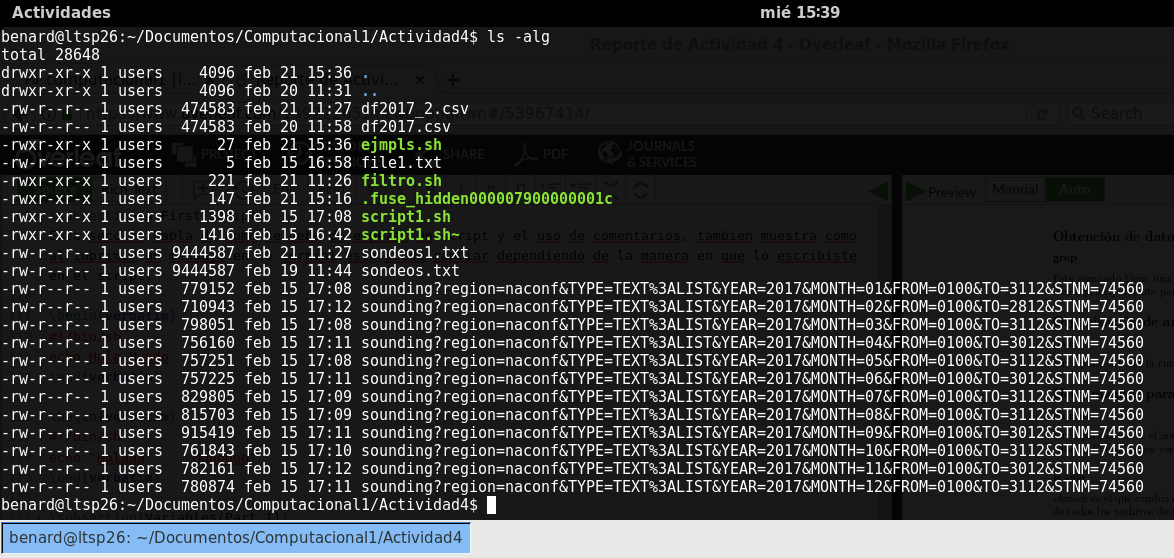
\includegraphics[width=12cm]{lsalg.png}
\end{center}
\vspace{0.3cm}

\subsubsection*{less}
Te muestra todo lo que está escrito en un archivo empezando desde el principio, es lo único que te muestra en la terminal, puedes terminar haciendo clic en q, y al regresar a la terminal normal no te muestra el archivo.

\subsubsection*{cat}
De igual manera que \textit{less}, \textit{cat} te muestra el contenido de un archivo, solo que en la terminal te manda de inmediato al final del archivo y este si se queda en la terminal.

\subsubsection*{diff}
Muestra la diferencia entre dos archivos.

\begin{center}
	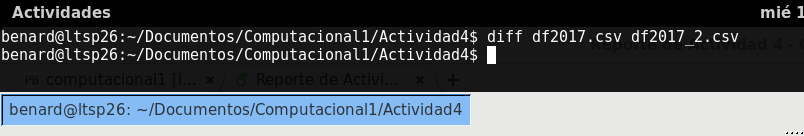
\includegraphics[width=12cm]{diff.png}
\end{center}
\vspace{0.3cm}

\subsubsection*{|}
Este es un separador, sirve para separar palabras o caracteres a la hora de buscar o filtrar varios.

\subsubsection*{>}
Sirve para mandar algo a un archivo, puede ser un conjunto de otros archivos, una palabra, número, etc.

\subsubsection*{wc}
Sirve para contar. Puede contar el número de líneas de un archivo, el número de caracteres y los bits de este.

\begin{center}
	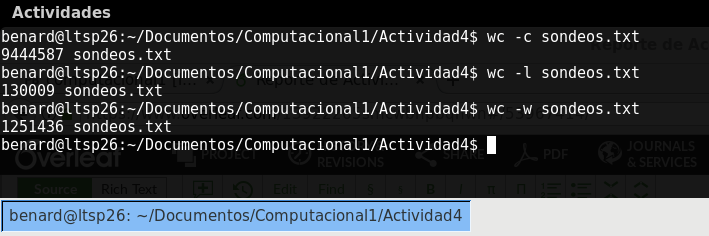
\includegraphics[width=12cm]{wc.png}
\end{center}
\vspace{0.3cm}


\section{Notas de Steve Parker: Síntesis}
En las referencias básicas de la practica aparece un link a un tutorial de Shell script con el cual pudimos crear el script que automatizara el proceso de hacer un archivo que tuviera los 12 archivos descargados y otro que filtrara este archivo. 

A continuación, esta una síntesis de los capítulos que me sirvieron para poder entender cómo funcionaba el script descargado al inicio de la práctica, y los que también me ayudaron a crear el script antes mencionado.

\subsection{Introduction}
En esta sección se nos habla un poco de que son los scripts y como surgieron. También nos enseñan como mandar desde la terminar algo a un script y como imprimir texto en la terminal desde un script.

\begin{verbatim}
echo 'echo Hola Mundo' > Ejm.sh
\end{verbatim}

\begin{verbatim}
#!/bin/sh
# Comentario
echo Hola Mundo 2.0	
\end{verbatim}

\subsection{Philosophy}
En esta sección se nos dice que para que un Shell script sea "bueno" este debe cumplir por lo menos con 2 características: que este "limpio" y fácil de leer, y evitar utilizar comandos innecesarios. Muestra un ejemplo de como un pequeño cambio en un código puede hacer que un programa corra más rápido.

\begin{verbatim}
#!/bin/sh
# Comentario
# Otro comentario 
echo Hola Mundo	
\end{verbatim}

\begin{verbatim}
#!/bin/sh
echo Hola Mundo	
\end{verbatim}

\subsection{A First Script}
Esta sección habla de cómo se debe de empezar un script y el uso de comentarios, también muestra como al imprimir un mensaje en la terminal este puede cambiar dependiendo de la manera en que lo escribiste en el script.

\begin{verbatim}
#!/bin/sh
echo Hola Mundo	
\end{verbatim}

\begin{verbatim}
#!/bin/sh
echo "Holaaa      Mundooo"	
\end{verbatim}

\subsection{Variables(Part 1)}
Nos muestran el uso de variables y de las maneras en que estas pueden, si es que puede, interactuar entre sí, esto dependiendo del contenido de la variable.

\begin{verbatim}
#!/bin/sh
Mensaje1="Hola Mundo"
echo $Mensaje1
\end{verbatim}

\begin{verbatim}
#!/bin/sh
Numero1=13
echo $Numero1
echo 19
echo 13 +19 =
expr $Numero1 + 19
\end{verbatim}

\subsection{Wildcards}
Esta sección habla de como el uso de una sintaxis diferente afecta el resultado del script.

\begin{verbatim}
#!/bin/sh
COPY=`cp /home/benard/Documentos/Computacional1/Actividad4/Ejemplos/*
.txt /home/benard/Documentos/Computacional1/Actividad4/EjmRes/`
echo $COPY
\end{verbatim}

\subsection{Escape Characters}
Esta sección nos enseña como imprimir caracteres que normalmente son usados como parte del codigo.

\begin{verbatim}
#!/bin/sh
echo "Hello   \"World\""
\end{verbatim}

\begin{verbatim}
#!/bin/sh
echo "*"
\end{verbatim}

\subsection{Loops}
En esta sección se nos introduce a los bucles (\textit{loops}), que son herramientas que se usan para repetir un proceso varias veces en lugar de escribir el mismo código varias veces.

\begin{verbatim}
#!/bin/sh
for i in 5 4 3 2 1
do
  echo "Autodestrucción en $i"
done
\end{verbatim}

\begin{verbatim}
#!/bin/sh
INPUT=Hallo
while [ "$INPUT" != "117" ]
do
  echo "Ingrese algo (117 para salir)"
  read INPUT
  echo "-----> $INPUT <-----"
done
\end{verbatim}

\subsection{Test}
Esta sección nos enseña el uso de los corchetes [ ], los cuales son un "programa" como ls, etc.

\begin{verbatim}
#!/bin/sh
echo "hi :]"
read X
if [ "$X" = "hi :]" ]
then
  echo ":D"
else
  echo "D:"
fi
\end{verbatim}

\begin{verbatim}
#!/bin/sh
echo Escribe un numero
read X
[ $X -ne 0 ] && echo "X isn't zero" || echo "X is zero"
\end{verbatim}

\subsection{Case}
En esta sección nos enseñan la manera en la que se escribe un pequeño codigo de \textit{Case}. Con estos uno puede prepararse para diferentes escenarios.

\begin{verbatim}
#!/bin/sh
echo "¿Como estas?"
while :
do
  read respuesta
  case $respuesta in
	bien)
		echo "Sehr gut!"
		;;
	mal)
		echo "):"
		echo "Why?"
		;;
	bye)
    	echo
		echo "bon voyage!"
		break
		;;
	adios)
		echo "bon voyage!"
		break
		;;
	*)
		echo "Soy un robot, no te entiendo"
		echo ":/"
		;;
  esac
done
\end{verbatim}

\begin{verbatim}
#!/bin/sh
echo "4 + 3 x 5 - 2= ??"
while :
do
  read respuesta
  case $respuesta in
	17)
		echo "Sehr gut!"
		echo
		break
		;;
	58)
		echo "No, sigue la jerarquía de operaciones."
		;;
	36)
		echo "No, sigue la jerarquía de operaciones."
		;;
	13)
		echo "No, sigue la jerarquía de operaciones."
		;;
	*)
		echo "How??"
		;;
  esac
done
\end{verbatim}

\subsection{Variables(Part 2)}
En esta sección nos muestran un conjunto de variables predeterminadas a las que no se les puede cambiar el valor.

\begin{verbatim}
#!/bin/sh
echo "I was called with $# parameters"
echo "My name is $0"
echo "My first parameter is $1"
echo "My second parameter is $2"
echo "All parameters are $@"
\end{verbatim}

\begin{verbatim}
#!/bin/sh
old_IFS="$IFS"
IFS=:
echo "Please input some data separated by colons (:)"
read x y z
IFS=$old_IFS
echo "x is $x y is $y z is $z"
\end{verbatim}

\subsection{Variables(Part 3)}
En esta sección nos enseñan como escribir en la terminal sin que automaticamente se le agrege un \textit{linebreak} al texto.


\begin{verbatim}
#!/bin/sh
echo -en "What is your name [ `whoami` ] "
read myname
if [ -z "$myname" ]; then
  myname=`whoami`
fi
echo "Your name is : $myname"
\end{verbatim}

\begin{verbatim}
#!/bin/sh
echo -en "What is your name [ `whoami` ] "
read myname
echo "Your name is : ${myname:-`whoami`}"
\end{verbatim}

\subsection{External Programs}
En esta sección se nos introduce a grep, uno de los programas "externos" que son comando que no están incorporados en Shell. Este lo usamos principalmente para filtrar, aunque tiene mucho otros usos.

\begin{verbatim}
#!/bin/sh
GREP=`grep -w PRES sounding\?region\=naconf\&TYPE\=TEXT%3ALIST\
&YEAR\=2017\&MONTH\=01\&FROM\=0100\&TO\=3112\&STNM\=74560`
echo $GREP
\end{verbatim}

\begin{verbatim}
#!/bin/sh
GREP=`grep -R "Texto de prueba" /home/benard/Documentos/
Computacional1/Actividad4`
echo $GREP
#Aparecera este archivo
\end{verbatim}

\subsection{Functions}
En esta sección nos muestran que los Shell scripts tambien pueden ser muy utiles a la hora de hacer funciones, e incluye varios ejemplos.

\begin{verbatim}
#!/bin/sh
# A simple script with a function...

add_a_user()
{
  USER=$1
  PASSWORD=$2
  shift; shift;
  # Having shifted twice, the rest is now comments ...
  COMMENTS=$@
  echo "Adding user $USER ..."
  echo useradd -c "$COMMENTS" $USER
  echo passwd $USER $PASSWORD
  echo "Added user $USER ($COMMENTS) with pass $PASSWORD"
}

###
# Main body of script starts here
###
echo "Start of script..."
add_a_user bob letmein Bob Holness the presenter
add_a_user fred badpassword Fred Durst the singer
add_a_user bilko worsepassword Sgt. Bilko the role model
echo "End of script..."
\end{verbatim}

\begin{verbatim}
#!/bin/sh
echo Factorial
factorial()
{
  if [ "$1" -gt "1" ]; then
    i=`expr $1 - 1`
    j=`factorial $i`
    k=`expr $1 \* $j`
    echo $k
  else
    echo 1
  fi
}


while :
do
  echo "Enter a number:"
  read x
  factorial $x
done  
\end{verbatim}

\subsection{Hints and Tips}
Como el nombre de esta sección sugiere, nos muestran unos cuantos tips al usar ciertos comandos.

\begin{verbatim}
#!/bin/sh
steves=`grep -i steve /etc/passwd | cut -d: -f1`
echo "All users with the word "steve" in their passwd"
echo "Entries are: "
echo "$steves" | tr ' ' '\012' | tr '[a-z]' '[A-Z]'
\end{verbatim}

\begin{verbatim}
#!/bin/sh
host=127.0.0.1
port=23
login=steve
passwd=hellothere
cmd="ls /tmp"

echo open ${host} ${port}
sleep 1
echo ${login}
sleep 1
echo ${passwd}
sleep 1
echo ${cmd}
sleep 1
echo exit
\end{verbatim}

\subsection{Quick Reference}
Esta sección es nos muestran una lista de comandos y variables con una pequeña descripsion de que hacen o que significan.


\section{Conclusíon}
Los programas (scripts) pueden ser de gran ayuda al automatizar diferentes procesos a la hora de trabajar con una gran cantidad de datos. No solo hacen el proceso de obtener, organizar y filtrar datos más fácil, sino mucho más rápido en comparación a hacerlo de otra manera.


\section{Bilbiografía}

\begin{verbatim}
Shell Scripting Tutorial. (n.d.). Retrieved February 21, 2018, 
from https://www.shellscript.sh/external.html 
\end{verbatim}
%https://www.shellscript.sh/external.html

\begin{verbatim}
Shell script. (2018, February 18). Retrieved February 21, 2018, 
from https://en.wikipedia.org/wiki/Shell_script 
\end{verbatim}
%https://en.wikipedia.org/wiki/Shell_script

\section{Apéndice}

			1.- ¿Qué fue lo que más te llamó la atención en esta actividad?
    
    \vspace{0.3cm}
 	Lo sencillo que es el crear un script que automatice diferentes procesos.
    \vspace{0.3cm}
    
\noindent    2.- ¿Qué consideras que aprendiste?
    
    \vspace{0.3cm}
    Varios comandos nuevos para las terminales y el uso de Shell scripts para automatizar el proceso de recolectar, organizar, y seleccionar información.
    \vspace{0.3cm}
    
\noindent    3.- ¿Cuáles fueron las cosas que más se te dificultaron?
    
    \vspace{0.3cm}
    Al principio pensé que sería difícil el crear el script que automatizara los puntos 13, 14 y 15 de la práctica, pero después de leer tutorial de Shell scripting me di cuenta que era mucho más fácil de lo parecía.
    \vspace{0.3cm}
    
\noindent    4.- ¿Cómo se podría mejorar en esta actividad?
    
    \vspace{0.3cm}
    En general, me pareció muy bien explicada.
    \vspace{0.3cm}
    
\noindent    5.- ¿En general, cómo te sentiste al realizar en esta actividad? 
    
    \vspace{0.3cm}
    Al principio un poco extrañado, pero este sentimiento se fue rápidamente.
    \vspace{0.3cm}


\end{document}